% ======= TABLA DE CONSULTAS =======
% Paquetes requeridos: booktabs, float, multirow
\begin{table}[H]
\centering
\caption{Tiempo promedio y desviación estándar (ns) por modelo RMQ.}
\renewcommand{\arraystretch}{1.2}
\setlength{\tabcolsep}{4pt}
\begin{tabular}{rcccccccc}
\toprule
\multirow{2}{*}{\textbf{Tamaño}} & \multicolumn{2}{c}{\textbf{ST-Static}} & \multicolumn{2}{c}{\textbf{ST-Dynamic}} & \multicolumn{2}{c}{\textbf{Seg-Static}} & \multicolumn{2}{c}{\textbf{Seg-Dynamic}}\\
\cmidrule(lr){2-3}\cmidrule(lr){4-5}\cmidrule(lr){6-7}\cmidrule(lr){8-9}
 & \textbf{Prom.} & \textbf{Desv.} & \textbf{Prom.} & \textbf{Desv.} & \textbf{Prom.} & \textbf{Desv.} & \textbf{Prom.} & \textbf{Desv.}\\
\midrule
1000 & 83.76 & 20.55 & 87.20 & 24.64 & 416.42 & 1019.32 & 441.75 & 180.37\\
2000 & 89.49 & 22.13 & 93.56 & 24.80 & 452.67 & 449.37 & 524.72 & 412.67\\
3000 & 92.30 & 21.72 & 96.32 & 26.53 & 492.52 & 192.51 & 562.20 & 375.79\\
4000 & 94.93 & 138.53 & 96.67 & 25.77 & 501.42 & 104.54 & 587.82 & 541.48\\
5000 & 84.25 & 19.75 & 103.51 & 29.52 & 514.22 & 233.87 & 602.46 & 127.51\\
\bottomrule
\end{tabular}
\end{table}

% ======= GRAFICO PGFPLOTS (SIN DESVIACIÓN ESTÁNDAR) =======
% Paquetes requeridos: pgfplots, xcolor
\begin{figure}[H]
\centering
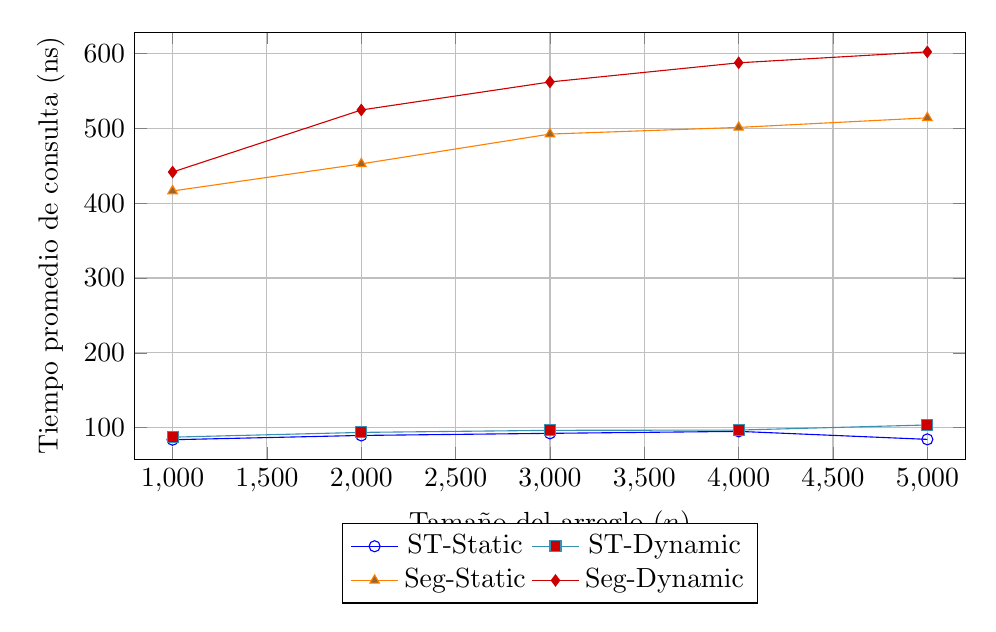
\begin{tikzpicture}
\begin{axis}[
  width=\textwidth,
  height=7cm,
  xlabel={Tamaño del arreglo ($n$)},
  ylabel={Tiempo promedio de consulta (ns)},
  grid=major,
  legend style={at={(0.5,-0.15)},anchor=north,legend columns=2},
  yticklabel style={/pgf/number format/fixed},
  enlargelimits=0.05
]
\addplot+[mark=o, color=blue] coordinates {
(1000,83.76133333333334)
(2000,89.48766666666667)
(3000,92.30333333333333)
(4000,94.92933333333333)
(5000,84.247)
};
\addlegendentry{ST-Static}
\addplot+[mark=square*, color=cyan!70!black] coordinates {
(1000,87.20266666666667)
(2000,93.56)
(3000,96.31633333333333)
(4000,96.67033333333333)
(5000,103.50566666666667)
};
\addlegendentry{ST-Dynamic}
\addplot+[mark=triangle*, color=orange] coordinates {
(1000,416.42333333333335)
(2000,452.6743333333333)
(3000,492.522)
(4000,501.4216666666667)
(5000,514.2233333333334)
};
\addlegendentry{Seg-Static}
\addplot+[mark=diamond*, color=red!80!black] coordinates {
(1000,441.74733333333336)
(2000,524.7246666666666)
(3000,562.2023333333333)
(4000,587.8166666666667)
(5000,602.456)
};
\addlegendentry{Seg-Dynamic}
\end{axis}
\end{tikzpicture}
\caption{Comparación del tiempo promedio de consulta para distintas estructuras RMQ.}
\end{figure}
